\documentclass{standalone}
\usepackage{tikz}
\usetikzlibrary{patterns, positioning}


\begin{document}
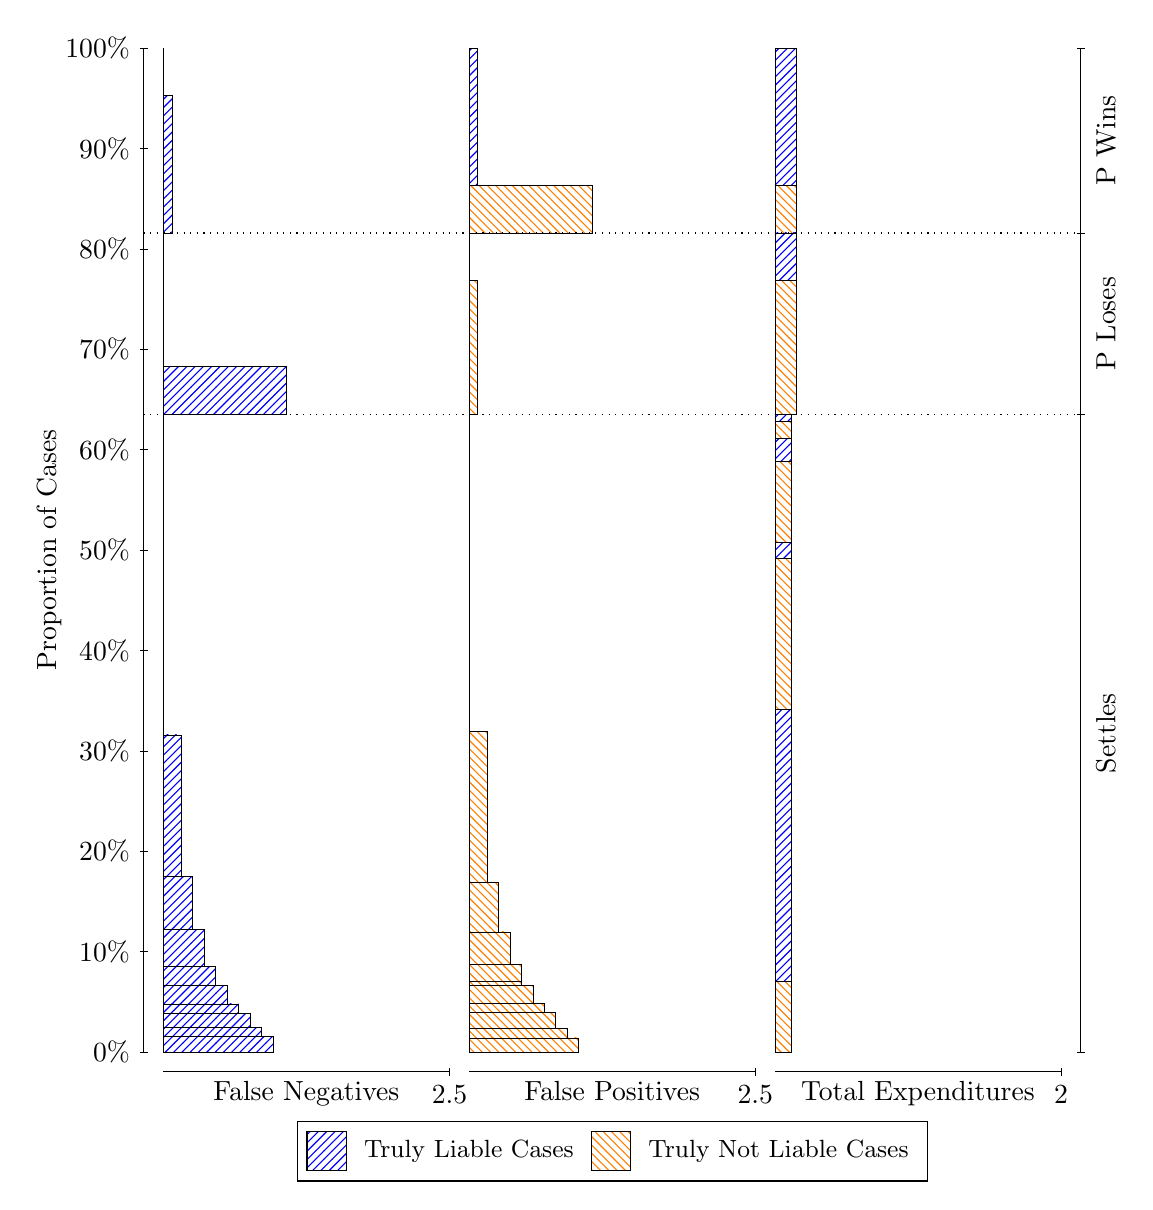
\begin{tikzpicture}
\draw[black, very thin] (1.5,1.75) -- (1.5,14.5);
\node[rotate=90, text=black, anchor=center] at (0.3, 8.125) {Proportion of Cases};
\draw[black, very thin] (1.45,1.75) -- (1.55,1.75);
\node[text=black, anchor=east] at (1.45, 1.75) {0\%};
\draw[black, very thin] (1.45,3.025) -- (1.55,3.025);
\node[text=black, anchor=east] at (1.45, 3.025) {10\%};
\draw[black, very thin] (1.45,4.3) -- (1.55,4.3);
\node[text=black, anchor=east] at (1.45, 4.3) {20\%};
\draw[black, very thin] (1.45,5.575) -- (1.55,5.575);
\node[text=black, anchor=east] at (1.45, 5.575) {30\%};
\draw[black, very thin] (1.45,6.85) -- (1.55,6.85);
\node[text=black, anchor=east] at (1.45, 6.85) {40\%};
\draw[black, very thin] (1.45,8.125) -- (1.55,8.125);
\node[text=black, anchor=east] at (1.45, 8.125) {50\%};
\draw[black, very thin] (1.45,9.4) -- (1.55,9.4);
\node[text=black, anchor=east] at (1.45, 9.4) {60\%};
\draw[black, very thin] (1.45,10.675) -- (1.55,10.675);
\node[text=black, anchor=east] at (1.45, 10.675) {70\%};
\draw[black, very thin] (1.45,11.95) -- (1.55,11.95);
\node[text=black, anchor=east] at (1.45, 11.95) {80\%};
\draw[black, very thin] (1.45,13.225) -- (1.55,13.225);
\node[text=black, anchor=east] at (1.45, 13.225) {90\%};
\draw[black, very thin] (1.45,14.5) -- (1.55,14.5);
\node[text=black, anchor=east] at (1.45, 14.5) {100\%};

\draw[black, very thin] (13.4,1.75) -- (13.4,14.5);
\draw[black, very thin] (13.35,1.75) -- (13.45,1.75);
\node[anchor=west] at (13.35, 1.75) {};
\draw[black, very thin] (13.35,9.8487) -- (13.45,9.8487);
\node[anchor=west] at (13.35, 9.8487) {};
\draw[black, very thin] (13.35,12.151) -- (13.45,12.151);
\node[anchor=west] at (13.35, 12.151) {};
\draw[black, very thin] (13.35,14.5) -- (13.45,14.5);
\node[anchor=west] at (13.35, 14.5) {};

\draw[black, very thin, pattern color=blue, pattern=north east lines] (1.75,1.75) rectangle (3.1398,1.9476);
\draw[black, very thin, pattern color=blue, pattern=north east lines] (1.75,1.9476) rectangle (2.9944,2.065);
\draw[black, very thin, pattern color=blue, pattern=north east lines] (1.75,2.065) rectangle (2.8491,2.2388);
\draw[black, very thin, pattern color=blue, pattern=north east lines] (1.75,2.2388) rectangle (2.7037,2.3598);
\draw[black, very thin, pattern color=blue, pattern=north east lines] (1.75,2.3598) rectangle (2.5584,2.5917);
\draw[black, very thin, pattern color=blue, pattern=north east lines] (1.75,2.5917) rectangle (2.4131,2.8321);
\draw[black, very thin, pattern color=blue, pattern=north east lines] (1.75,2.8321) rectangle (2.2678,3.303);
\draw[black, very thin, pattern color=blue, pattern=north east lines] (1.75,3.303) rectangle (2.1224,3.9753);
\draw[black, very thin, pattern color=blue, pattern=north east lines] (1.75,3.9753) rectangle (1.9771,5.7761);
\draw[black, very thin, pattern color=orange, pattern=north west lines] (1.75,5.7761) rectangle (1.75,9.8487);
\draw[black, very thin, pattern color=blue, pattern=north east lines] (1.75,9.8487) rectangle (3.3123,10.452);
\draw[black, very thin, pattern color=orange, pattern=north west lines] (1.75,10.452) rectangle (1.75,12.151);
\draw[black, very thin, pattern color=blue, pattern=north east lines] (1.75,12.151) rectangle (1.859,13.896);
\draw[black, very thin, pattern color=orange, pattern=north west lines] (1.75,13.896) rectangle (1.75,14.5);
\draw[black, very thin, pattern color=orange, pattern=north west lines] (5.6333,1.75) rectangle (7.0231,1.9289);
\draw[black, very thin, pattern color=orange, pattern=north west lines] (5.6333,1.9289) rectangle (6.8777,2.0496);
\draw[black, very thin, pattern color=orange, pattern=north west lines] (5.6333,2.0496) rectangle (6.7324,2.2514);
\draw[black, very thin, pattern color=orange, pattern=north west lines] (5.6333,2.2514) rectangle (6.5871,2.3622);
\draw[black, very thin, pattern color=orange, pattern=north west lines] (5.6333,2.3622) rectangle (6.4417,2.5961);
\draw[black, very thin, pattern color=orange, pattern=north west lines] (5.6333,2.5961) rectangle (6.2964,2.6499);
\draw[black, very thin, pattern color=orange, pattern=north west lines] (5.6333,2.6499) rectangle (6.2964,2.8661);
\draw[black, very thin, pattern color=orange, pattern=north west lines] (5.6333,2.8661) rectangle (6.1511,3.2739);
\draw[black, very thin, pattern color=orange, pattern=north west lines] (5.6333,3.2739) rectangle (6.0057,3.9026);
\draw[black, very thin, pattern color=orange, pattern=north west lines] (5.6333,3.9026) rectangle (5.8604,5.8226);
\draw[black, very thin, pattern color=blue, pattern=north east lines] (5.6333,5.8226) rectangle (5.6333,9.8487);
\draw[black, very thin, pattern color=orange, pattern=north west lines] (5.6333,9.8487) rectangle (5.7423,11.547);
\draw[black, very thin, pattern color=blue, pattern=north east lines] (5.6333,11.547) rectangle (5.6333,12.151);
\draw[black, very thin, pattern color=orange, pattern=north west lines] (5.6333,12.151) rectangle (7.1957,12.755);
\draw[black, very thin, pattern color=blue, pattern=north east lines] (5.6333,12.755) rectangle (5.7423,14.5);
\draw[black, very thin, pattern color=orange, pattern=north west lines] (9.5167,1.75) rectangle (9.721,2.6499);
\draw[black, very thin, pattern color=blue, pattern=north east lines] (9.5167,2.6499) rectangle (9.721,6.1009);
\draw[black, very thin, pattern color=orange, pattern=north west lines] (9.5167,6.1009) rectangle (9.721,8.0209);
\draw[black, very thin, pattern color=blue, pattern=north east lines] (9.5167,8.0209) rectangle (9.721,8.2186);
\draw[black, very thin, pattern color=orange, pattern=north west lines] (9.5167,8.2186) rectangle (9.721,9.255);
\draw[black, very thin, pattern color=blue, pattern=north east lines] (9.5167,9.255) rectangle (9.721,9.5462);
\draw[black, very thin, pattern color=orange, pattern=north west lines] (9.5167,9.5462) rectangle (9.721,9.7624);
\draw[black, very thin, pattern color=blue, pattern=north east lines] (9.5167,9.7624) rectangle (9.721,9.8487);
\draw[black, very thin, pattern color=orange, pattern=north west lines] (9.5167,9.8487) rectangle (9.7892,11.547);
\draw[black, very thin, pattern color=blue, pattern=north east lines] (9.5167,11.547) rectangle (9.7892,12.151);
\draw[black, very thin, pattern color=orange, pattern=north west lines] (9.5167,12.151) rectangle (9.7892,12.755);
\draw[black, very thin, pattern color=blue, pattern=north east lines] (9.5167,12.755) rectangle (9.7892,14.5);
\draw[black, dotted] (1.5,9.8487) -- (13.4,9.8487);
\draw[black, dotted] (1.5,12.151) -- (13.4,12.151);
\draw[black, very thin] (1.75,1.5) -- (5.3833,1.5);
\node[text=black, anchor=north] at (3.5667, 1.5) {False Negatives};
\draw[black, very thin] (5.3833,1.45) -- (5.3833,1.55);
\node[text=black, anchor=north] at (5.3833, 1.45) {2.5};

\draw[black, very thin] (5.6333,1.5) -- (9.2667,1.5);
\node[text=black, anchor=north] at (7.45, 1.5) {False Positives};
\draw[black, very thin] (9.2667,1.45) -- (9.2667,1.55);
\node[text=black, anchor=north] at (9.2667, 1.45) {2.5};

\draw[black, very thin] (9.5167,1.5) -- (13.15,1.5);
\node[text=black, anchor=north] at (11.333, 1.5) {Total Expenditures};
\draw[black, very thin] (13.15,1.45) -- (13.15,1.55);
\node[text=black, anchor=north] at (13.15, 1.45) {2};

\node[text=black, centered, rotate=90] at (13.72, 5.7993) {Settles};
\node[text=black, centered, rotate=90] at (13.72, 11) {P Loses};
\node[text=black, centered, rotate=90] at (13.72, 13.325) {P Wins};

\draw (7.449999999999999,1.5) node[draw=none] (baseCoordinate) {};
\begin{scope}[align=center]
        \matrix[scale=0.5, draw=black, below=0.5cm of baseCoordinate, nodes={draw}, column sep=0.1cm]{
            \node[rectangle, draw, minimum width=0.5cm, minimum height=0.5cm, pattern color=blue, pattern=north east lines] {}; &
            \node[draw=none, font=\small, text=black] (B) {Truly Liable Cases}; &
            \node[rectangle, draw, minimum width=0.5cm, minimum height=0.5cm, pattern color=orange, pattern=north west lines] {}; &
            \node[draw=none, font=\small, text=black] (B) {Truly Not Liable Cases}; \\
            };
\end{scope}

\end{tikzpicture}
\end{document}